\documentclass[border=5pt]{standalone}
\usepackage{tikz}
\usepackage{xcolor}
\usetikzlibrary{calc,shadows.blur}

% J4 - Pink thick ring
\begin{document}
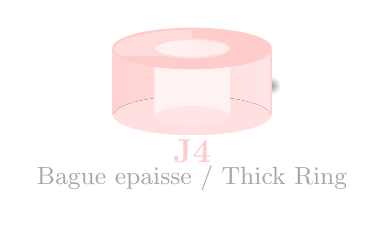
\begin{tikzpicture}

% Shadow
\fill[gray!25,blur shadow={shadow blur steps=5}] (0,-0.1) ellipse (1.0 and 0.18);

% Outer cylinder body (thick ring - 3D isometric-like)
% Bottom ellipse
\fill[pink!50] (0,-0.55) ellipse (1.0 and 0.25);
\fill[pink!40] (0,-0.55) ellipse (0.48 and 0.12);

% Side wall outer
\fill[left color=pink!70, right color=pink!40]
  (-1.0,-0.55) -- (-1.0,0.3) arc[start angle=180,end angle=0,x radius=1.0,y radius=0.25]
  -- (1.0,-0.55) arc[start angle=0,end angle=180,x radius=1.0,y radius=0.25];

% Side wall inner hole
\fill[pink!20]
  (-0.48,-0.55) -- (-0.48,0.3) arc[start angle=180,end angle=0,x radius=0.48,y radius=0.12]
  -- (0.48,-0.55) arc[start angle=0,end angle=180,x radius=0.48,y radius=0.12];

% Top face (annular ring)
\fill[pink!80] (0,0.3) ellipse (1.0 and 0.25);
\fill[pink!30] (0,0.3) ellipse (0.48 and 0.12);

% Highlight on top
\begin{scope}
  \clip (0,0.3) ellipse (1.0 and 0.25);
  \fill[white,opacity=0.3] (-1.1,0.2) rectangle (0,0.6);
\end{scope}

% Outlines
\draw[pink!80, line width=0.8pt] (0,0.3) ellipse (1.0 and 0.25);
\draw[pink!60, line width=0.6pt] (0,0.3) ellipse (0.48 and 0.12);
\draw[pink!70, line width=0.8pt] (-1.0,-0.55) -- (-1.0,0.3);
\draw[pink!70, line width=0.8pt] (1.0,-0.55) -- (1.0,0.3);

% Label
\node[font=\bfseries\large, text=pink!80] at (0,-1.0) {J4};
\node[font=\small, text=gray!70] at (0,-1.35) {Bague epaisse / Thick Ring};

\end{tikzpicture}
\end{document}
